\newpage
\section{地形データの収集方法}
\label{sec:method1}

\subsection{地形生成の手法}
本研究では,効率的に未知環境の地形を収集する手法として,生成AIを用いた地形のメッシュデータを生成をする方法を提案する.
生成AIのモデルにはGANを三次元のボクセルベースに応用した3D-IWGANを用いた.\cite{bunken1}

\subsection{詳細手順}
最初にGANの学習用データとしてNASAの提供している月面のメッシュデータを用意した.25種類のデータがあるが,それを表面に沿って4\times4に分割することで学習データ拡張を行った.拡張後の各データに対し,地形表面のメッシュ三角形から頂点座標を抽出し,それを元にボクセル化を行う.このボクセルの三次元座標データをGANの入力として学習させ,新たな三次元座標データを生成させる.次にこの座標をスプライン曲線で補間し,得られた点を頂点とした三角形メッシュで埋めることで最終的な不整地データを作成する.

\subsubsection{NASAの月面データについて}
上記で説明した通り、NASAの提供している月面データを利用してデータセットにする.アポロ11号等の宇宙船が着陸した地点から$30 \mathrm{\, km}$\times$30\mathrm{\, km}$の範囲の高度マップになっている.これらは3Dプリンティング等のために提供されており,ファイルはSTL形式のメッシュデータになっている.以下の図\ref{fig:NASA_moons}に使用したデータの例を示す.

\begin{figure}[htbp]
    \centering
    \begin{minipage}[b]{0.48\linewidth}
      \centering
      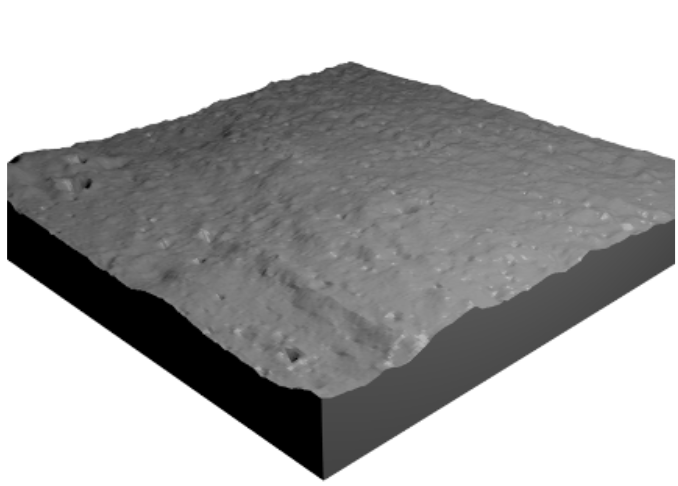
\includegraphics[keepaspectratio, scale=0.3]{images/NASA_moon.png}
      \subcaption{月面の例1}\label{fig:NASA_moon}
    \end{minipage}
    \begin{minipage}[b]{0.48\linewidth}
      \centering
      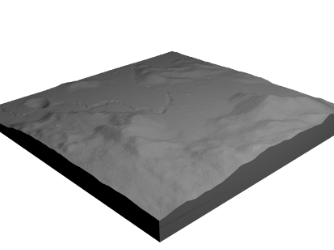
\includegraphics[keepaspectratio, scale=0.6]{images/NASA_moon2.png}
      \subcaption{月面の例2}\label{fig:NASA_moon2}
    \end{minipage}
    \begin{minipage}[b]{0.48\linewidth}
      \centering
      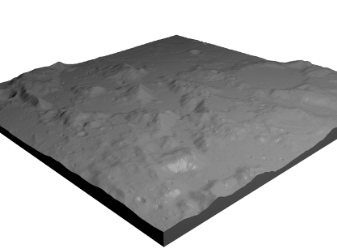
\includegraphics[keepaspectratio, scale=0.6]{images/NASA_moon3.png}
      \subcaption{月面の例3}\label{fig:NASA_moon3}
    \end{minipage}
    \begin{minipage}[b]{0.48\linewidth}
      \centering
      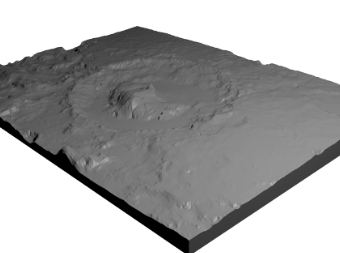
\includegraphics[keepaspectratio, scale=0.6]{images/NASA_moon5.png}
      \subcaption{月面の例4}\label{fig:NASA_moon5}
    \end{minipage}
    \begin{minipage}[b]{0.48\linewidth}
        \centering
        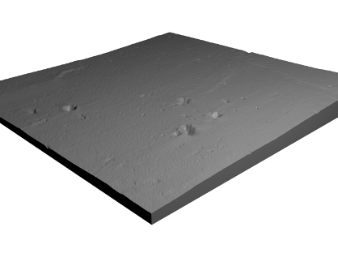
\includegraphics[keepaspectratio, scale=0.6]{images/NASA_moon6.png}
        \subcaption{月面の例5}\label{fig:NASA_moon6}
      \end{minipage}
      \begin{minipage}[b]{0.48\linewidth}
        \centering
        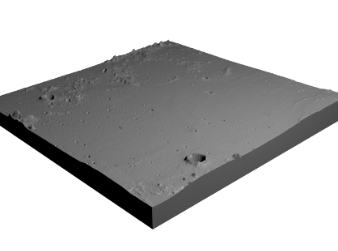
\includegraphics[keepaspectratio, scale=0.6]{images/NASA_moon7.png}
        \subcaption{月面の例6}\label{fig:NASA_moon7}
      \end{minipage}
    \caption{使用した月面の例}\label{fig:NASA_moons}
  \end{figure}

\subsubsection{ボクセル化について}
本研究では,三次元分布の可視化をする際にその特徴をボクセルによって表現することとした.このボクセルの解像度によって地表面の起伏度合いを調整できることと,その起伏度合いが視覚的に伝わりやすいためである.ここでは月面データをボクセル化する方法について具体的に述べていく.まずはボクセルの解像度を設定する.ここでは仮にボクセルの解像度を256\times256\times64とする.地表のメッシュ三角形の頂点座標を取得し[図\ref{fig:mesh1}],256\times256の各格子内にある頂点の平均値をその代表点とする.[図\ref{fig:mesh2}]それらの点の最大値が高さ方向の解像度の64マス目となる.このようにして0マス目からその格子の点の高さまでを点で埋めることで,0と1で表現された256\times256\times64の座標データが出来上がる.これに従って$1\mathrm{\,m}$\times$1\mathrm{\,m}$\times$1\mathrm{\,m}$の矩形を描くことでボクセルを表現する.

\begin{figure}[htbp]
    \begin{center}
     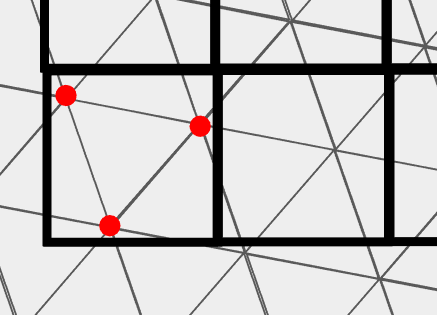
\includegraphics[width=0.5\linewidth]{images/mesh1.png}
     \caption{手順1}
     \label{fig:mesh1}
    \end{center}
\end{figure}

\begin{figure}[htbp]
    \begin{center}
     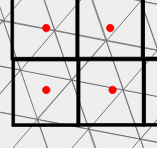
\includegraphics[width=0.5\linewidth]{images/mesh2.png}
     \caption{手順2}
     \label{fig:mesh2}
    \end{center}
\end{figure}

\subsubsection{GANを用いた地形データ生成について}
三次元ボクセルの高さ方向の分散により,不整地の起伏度合いを表現した.使用したGANモデルの構造を以下の図\ref{fig:3d_gan}に示す.データの入力方法は,正規分布に従った乱数の平均と標準偏差の値を入力する方法,画像をエンコードした後の平均と標準偏差の値を入力する方法,深度カメラ等を用いて取得した画像から作成した三次元のボクセル座標をエンコードした後,その平均と標準偏差の値を入力する方法の3種類となっている.月面データを32\times32\times32に分割したボクセルにし,その三次元座標をGANの入力として学習を行った出力結果が図\ref{fig:voxel}である.

\begin{figure}[htbp]
    \begin{center}
     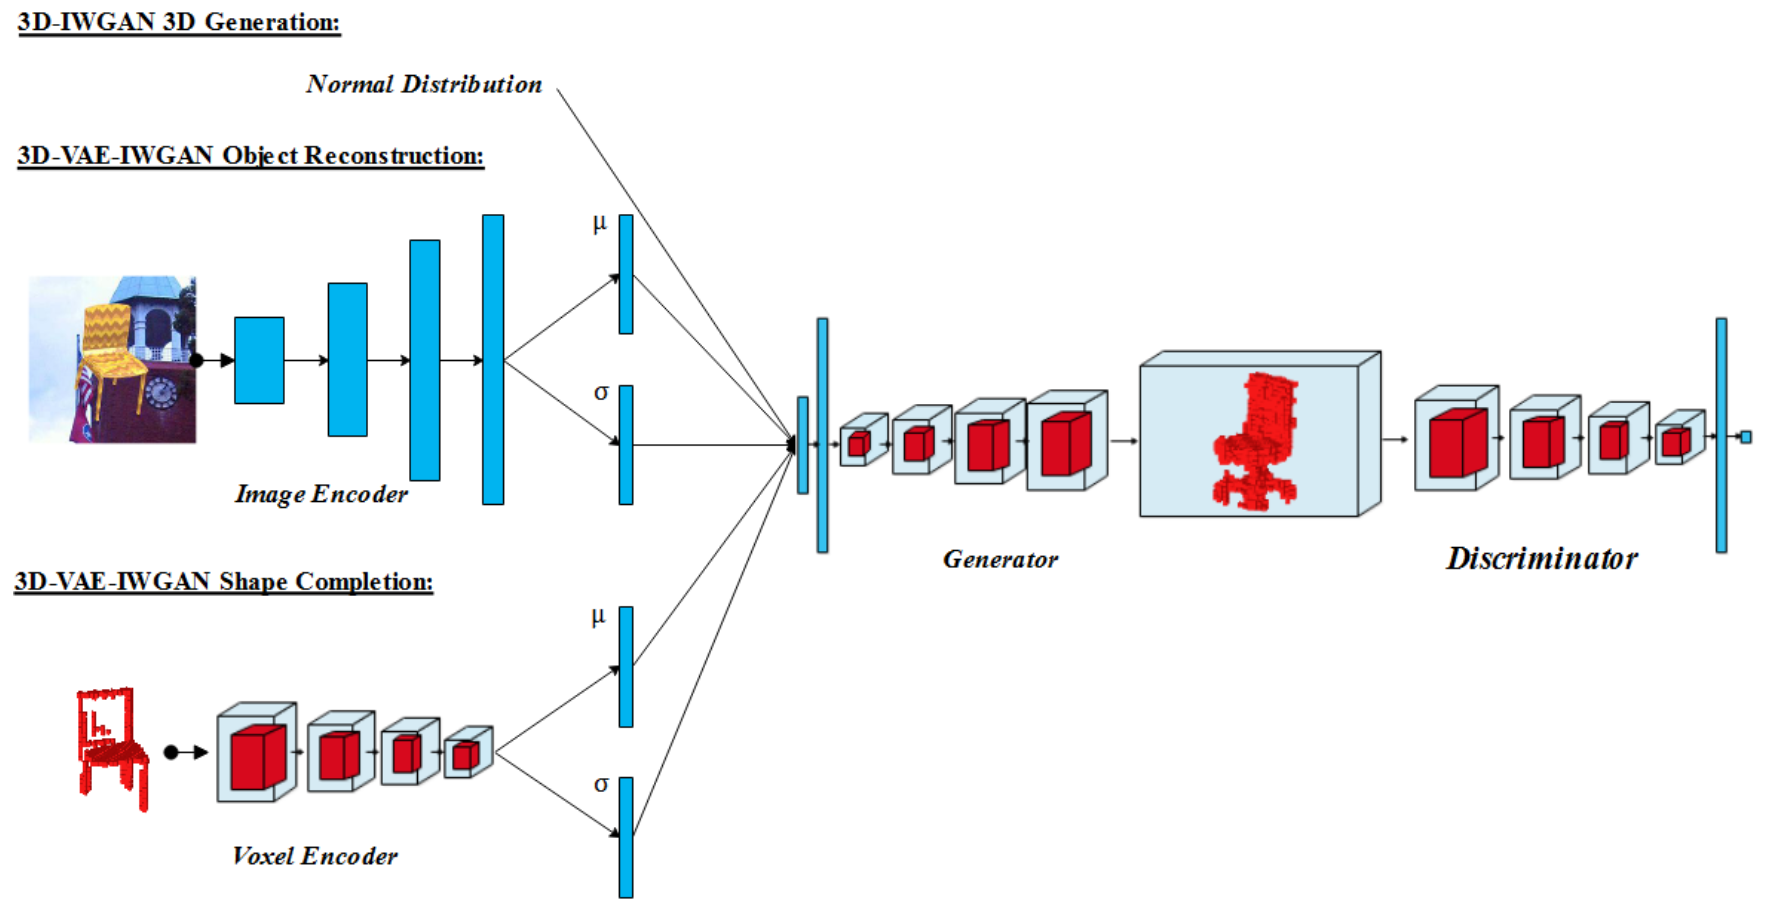
\includegraphics[width=1.0\linewidth]{images/3d_gan.png}
     \caption{3D-IWGANのモデル構造}
     \label{fig:3d_gan}
    \end{center}
\end{figure}

\begin{figure}[htbp]
    \begin{center}
     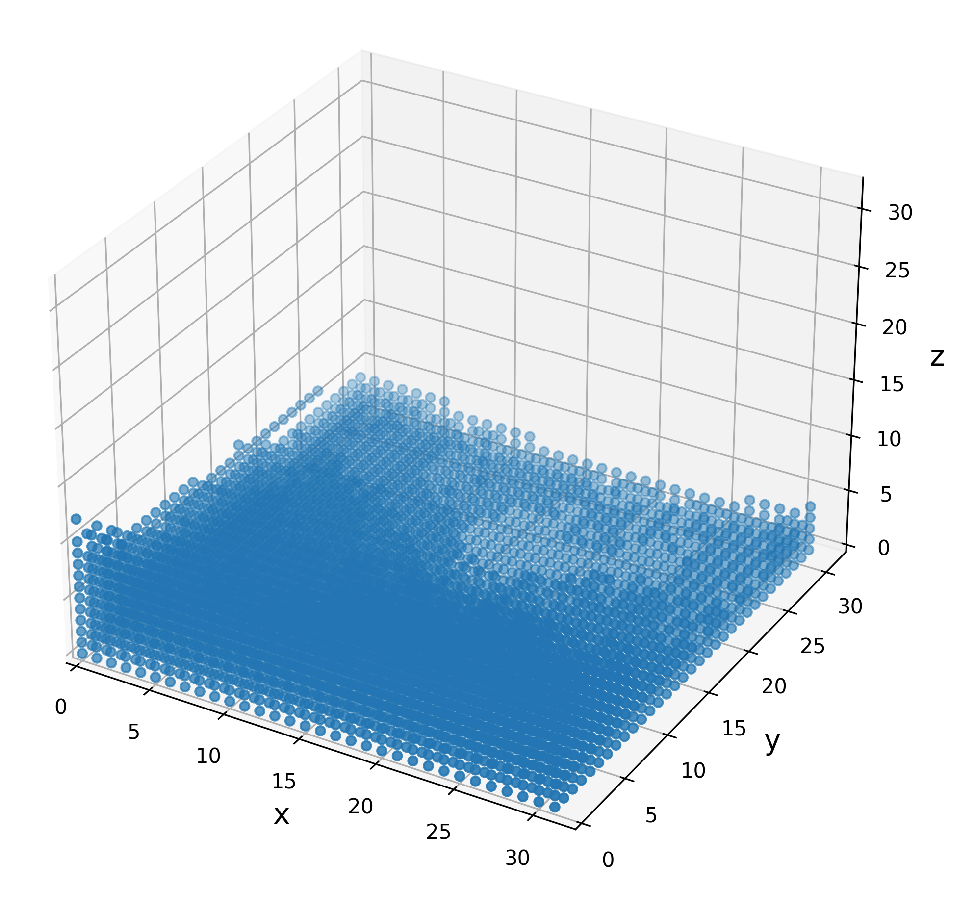
\includegraphics[width=0.6\linewidth]{images/voxel.png}
     \caption{GANでの学習結果}
     \label{fig:voxel}
    \end{center}
\end{figure}

\subsubsection{メッシュ化について}
ボクセル化した地形を元の月面のようになだらかな地表に変換するため,本研究ではボクセルの点からスプライン補間\cite{bunken3}によって求めた曲線に基づいてメッシュデータに変換する方法を用いた.スプライン補間はある複数の点を全て通る曲線の多項式を求める方法である.仮にxy平面の三次のスプライン補間を行う場合,以下のような多項式になる.ここでSは曲線が通る各点のy座標,nは曲線が通る点の数,そして最終的に求めるのは各項の係数となる.\\
\begin{math}
    S_0(x)  = a_0 + b_0(x - x_0) + c_0(x - x_0)^{2} + d_0(x - x_0)^{3}\\
    S_1(x)  = a_1 + b_1(x - x_1) + c_1(x - x_1)^{2} + d_1(x - x_1)^{3}\\
    S_2(x)  = a_2 + b_2(x - x_2) + c_2(x - x_2)^{2} + d_2(x - x_2)^{3}\\
    \vdots\\
    S_j(x)  = a_j + b_j(x - x_j) + c_j(x - x_j)^{2} + d_j(x - x_j)^{3}\\
    \vdots\\
    S_{n-1}(x)  = a_{n-1} + b_{n-1}(x - x_{n-1}) + c_{n-1}(x - x_{n-1})^{2} + d_{n-1}(x - x_{n-1})^{3}\\
\end{math}
生成した地形では次数を10と設定したため,多項式は以下のようになり,求める係数は
\begin{math}a \sim k\end{math}
となる.\\
\begin{math}
    S_{n-1}(x)  = a_{n-1} + b_{n-1}(x - x_{n-1}) + c_{n-1}(x - x_{n-1})^{2} + d_{n-1}(x - x_{n-1})^{3}\ldots + k_{n-1}(x - x_{n-1})^{10}
\end{math}

これにはPythonの数値解析ライブラリであるSciPyからscipy.interpolate.bisplrepという関数を呼び出すことで自動で計算を行った.
この曲線にそって三角形メッシュの頂点を決定してメッシュ化を行う.以下の図\ref{fig:mesh_moons}は生成した月面のボクセルデータとそれを元にメッシュ化した月面データの例である.高さの離れた点が隣接していると,スプライン曲線の特性上例の4のように極端に鋭利な地形領域ができてしまう場合があった.

\begin{figure}[htbp]
    \centering
    \begin{minipage}[b]{0.49\linewidth}
      \centering
      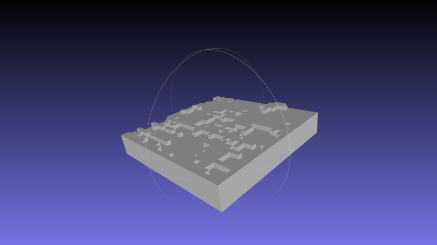
\includegraphics[keepaspectratio, scale=0.45]{images/voxel1.png}
      \subcaption{ボクセル化した月面の例1}\label{fig:voxel1}
    \end{minipage}
    \begin{minipage}[b]{0.49\linewidth}
      \centering
      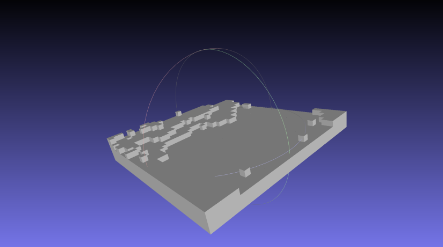
\includegraphics[keepaspectratio, scale=0.45]{images/voxel2.png}
      \subcaption{ボクセル化した月面の例2}\label{fig:voxel2}
    \end{minipage}
    \begin{minipage}[b]{0.49\linewidth}
      \centering
      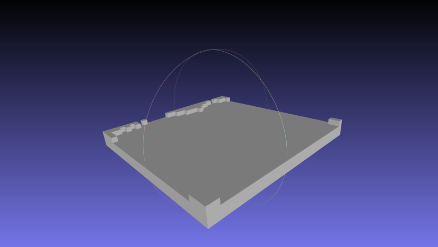
\includegraphics[keepaspectratio, scale=0.45]{images/voxel3.png}
      \subcaption{ボクセル化した月面の例3}\label{fig:voxel3}
    \end{minipage}
    \begin{minipage}[b]{0.49\linewidth}
      \centering
      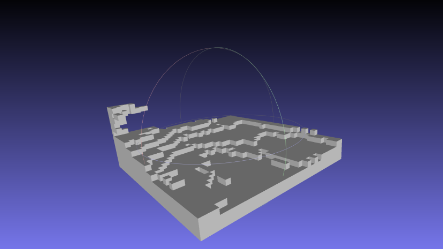
\includegraphics[keepaspectratio, scale=0.45]{images/voxel4.png}
      \subcaption{ボクセル化した月面の例4}\label{fig:voxel4}
    \end{minipage}
    \begin{minipage}[b]{0.49\linewidth}
        \centering
        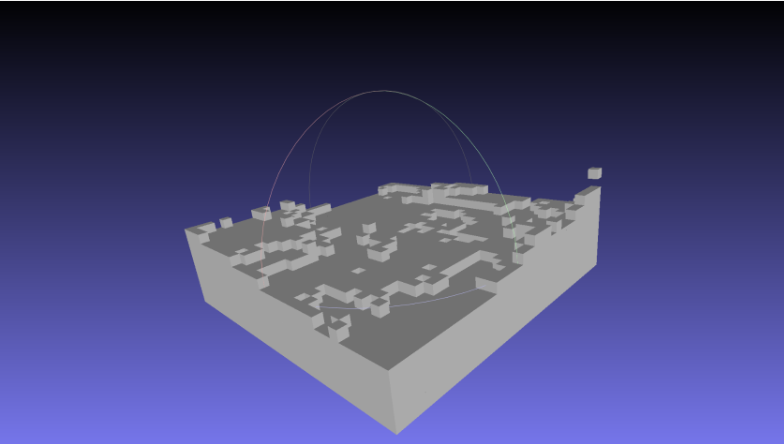
\includegraphics[keepaspectratio, scale=0.245]{images/voxel5.png}
        \subcaption{ボクセル化した月面の例5}\label{fig:voxel5}
      \end{minipage}
    \begin{minipage}[b]{0.49\linewidth}
    \centering
    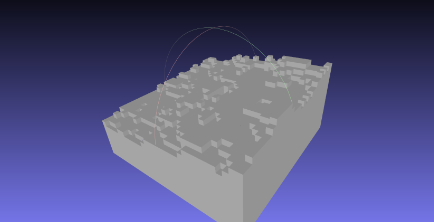
\includegraphics[keepaspectratio, scale=0.45]{images/voxel6.png}
    \subcaption{ボクセル化した月面の例6}\label{fig:voxel6}
    \end{minipage}
    \begin{minipage}[b]{0.49\linewidth}
    \centering
    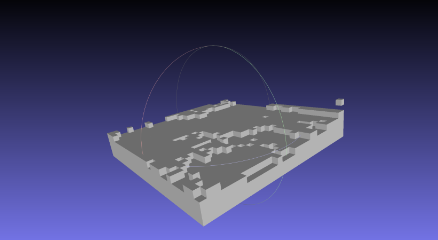
\includegraphics[keepaspectratio, scale=0.45]{images/voxel7.png}
    \subcaption{ボクセル化した月面の例7}\label{fig:voxel7}
    \end{minipage}
    \begin{minipage}[b]{0.49\linewidth}
    \centering
    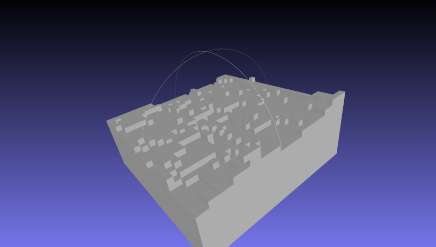
\includegraphics[keepaspectratio, scale=0.45]{images/voxel8.png}
    \subcaption{ボクセル化した月面の例8}\label{fig:voxel8}
    \end{minipage}
    \caption{ボクセル化した月面の例}\label{fig:voxel_moons}
  \end{figure}

  \begin{figure}[htbp]
    \centering
    \begin{minipage}[b]{0.49\linewidth}
      \centering
      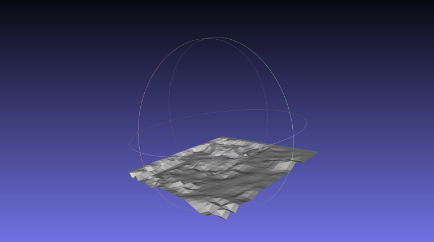
\includegraphics[keepaspectratio, scale=0.47]{images/spline1.png}
      \subcaption{メッシュ化した月面の例1}\label{fig:spline1}
    \end{minipage}
    \begin{minipage}[b]{0.49\linewidth}
      \centering
      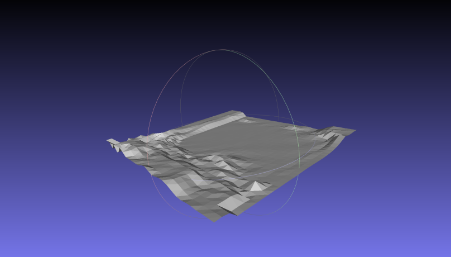
\includegraphics[keepaspectratio, scale=0.45]{images/spline2.png}
      \subcaption{メッシュ化した月面の例2}\label{fig:spline2}
    \end{minipage}
    \begin{minipage}[b]{0.49\linewidth}
      \centering
      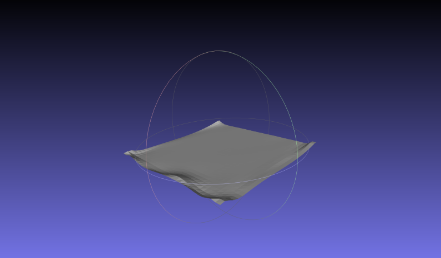
\includegraphics[keepaspectratio, scale=0.45]{images/spline3.png}
      \subcaption{メッシュ化した月面の例3}\label{fig:spline3}
    \end{minipage}
    \begin{minipage}[b]{0.49\linewidth}
      \centering
      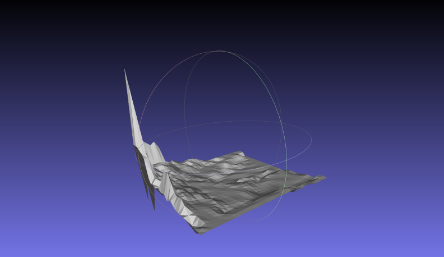
\includegraphics[keepaspectratio, scale=0.45]{images/spline4.png}
      \subcaption{メッシュ化した月面の例4}\label{fig:spline4}
    \end{minipage}
    \begin{minipage}[b]{0.49\linewidth}
        \centering
        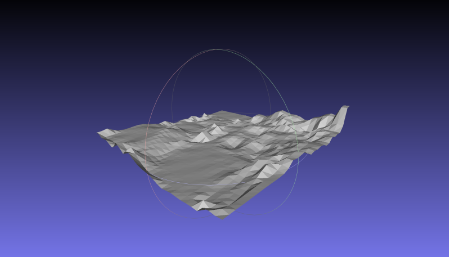
\includegraphics[keepaspectratio, scale=0.44]{images/spline5.png}
        \subcaption{メッシュ化した月面の例5}\label{fig:spline5}
      \end{minipage}
      \begin{minipage}[b]{0.49\linewidth}
        \centering
        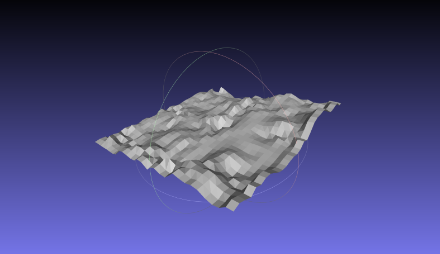
\includegraphics[keepaspectratio, scale=0.45]{images/spline6.png}
        \subcaption{メッシュ化した月面の例6}\label{fig:spline6}
      \end{minipage}
      \begin{minipage}[b]{0.49\linewidth}
        \centering
        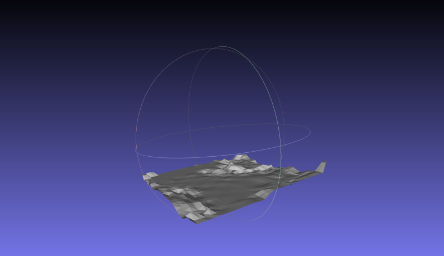
\includegraphics[keepaspectratio, scale=0.45]{images/spline7.png}
        \subcaption{メッシュ化した月面の例7}\label{fig:spline7}
      \end{minipage}
      \begin{minipage}[b]{0.49\linewidth}
        \centering
        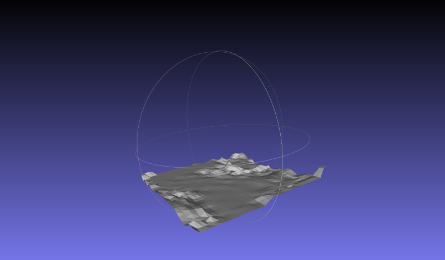
\includegraphics[keepaspectratio, scale=0.45]{images/spline8.png}
        \subcaption{メッシュ化した月面の例8}\label{fig:spline8}
      \end{minipage}
    \caption{スプライン近似によってメッシュ化した月面の例}\label{fig:mesh_moons}
  \end{figure}